% Extensión estimada: unas 5 páginas, cuatro subsecciones, tres tablas y cuatro figuras (ficha 4.2).
% Fuentes: ficha fichas/04-resultados-clasificacion/02-evaluaciones-complementarias.md; Codigo/outputs/results/
% hiba_por_modalidad.json y *_les_cwnone_hiba_predictions_hiba.json; robustness/robustness_summary.json;
% lesion_split_report.json (calibracion) y calibration_les/calibration_summary.json;
% interpretability_les/interpretability_swin.png. Figuras: scripts/figuras_cap4.py y scripts/figura_gradcam_tesina.py.
% El costo pasó a sec:res_comparacion (revisión del autor, 24/10/2026).
\section{Evaluaciones complementarias del clasificador}
\label{sec:res_complementarios}

La prueba de \emph{HAM10000} comparte población, equipo de captura y forma de etiquetar con el entrenamiento. Cuatro de
las evaluaciones de la Sección~\ref{sec:met_complementarios} cambian esas condiciones o examinan otros aspectos del
clasificador: otra población, imágenes degradadas, la confianza de sus probabilidades y la región en que se apoya. La
quinta, el costo, se presenta junto con la comparación de la Sección~\ref{sec:res_comparacion}. Se evalúa Swin-Tiny
con la semilla 42, y las tablas incluyen a ConvNeXt-Tiny como contraste.

\subsection{Generalización a otra población}
\label{sec:res_hiba}

Sin ningún ajuste, en las 1\,616 imágenes de \emph{HIBA} la sensibilidad macro de Swin-Tiny cae de 0.716 a 0.424
(Tabla~\ref{tab:res_hiba}). La caída es mayor en las fotografías clínicas, una modalidad que el modelo no vio en el
entrenamiento, pero aparece también en las imágenes dermatoscópicas. ConvNeXt-Tiny cae de manera parecida.

\begin{table}[H]
    \centering
    \caption{Sensibilidad macro en la prueba de \emph{HAM10000} y en \emph{HIBA}, por modalidad.}
    \label{tab:res_hiba}
    \small
    \setlength{\tabcolsep}{4pt}
    \begin{tabularx}{\textwidth}{@{}>{\raggedright\arraybackslash}X
        >{\centering\arraybackslash}p{2.3cm}>{\centering\arraybackslash}p{1.9cm}
        >{\centering\arraybackslash}p{2.9cm}>{\centering\arraybackslash}p{1.9cm}@{}}
        \toprule
        & & \multicolumn{3}{c}{\textbf{\emph{HIBA}}} \\
        \cmidrule(l){3-5}
        \textbf{Modelo} & \textbf{\emph{HAM10000}} & \textbf{Total} & \textbf{Dermatoscópicas} & \textbf{Clínicas} \\
        \midrule
        Imágenes & 1\,503 & 1\,616 & 1\,270 & 346 \\
        \midrule
        Swin-Tiny & 0.716 & 0.424 & 0.494 & 0.236 \\
        ConvNeXt-Tiny & 0.694 & 0.447 & 0.519 & 0.263 \\
        \bottomrule
    \end{tabularx}
\end{table}

La Figura~\ref{fig:res_hiba_clases} muestra que la caída alcanza a todas las clases salvo \gls{nv}, que se sostiene.
La más afectada es \gls{akiec}, en la que influye el mapeo de diagnósticos de la Sección~\ref{sec:met_hiba}: 158 de
sus 221 imágenes en \emph{HIBA} son carcinomas escamosos, un ruido que no puede separarse del cambio de población. Sin
embargo, también \gls{mel} pierde un tercio de su sensibilidad, y \gls{bcc}, más de la mitad. Por lo tanto, el
desempeño medido en \emph{HAM10000} no se traslada a esta población, aun dentro de la misma modalidad.

\begin{figure}[H]
    \centering
    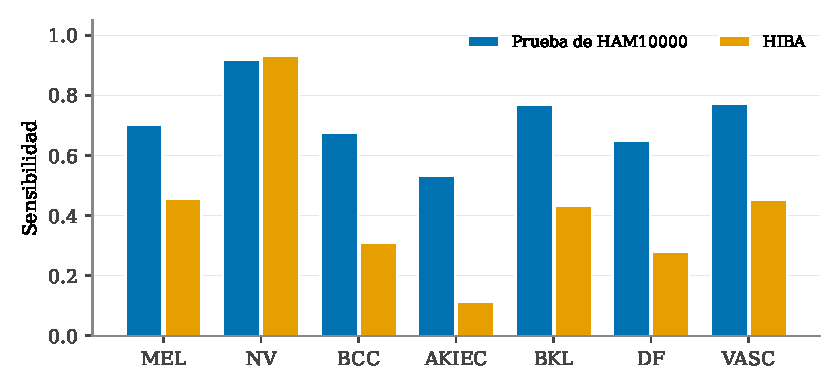
\includegraphics[width=0.85\textwidth]{Figures/Capitulos/04-Resultados-Clasificacion/hiba-por-clase-swin.pdf}
    \caption{Sensibilidad por clase de Swin-Tiny en la prueba de \emph{HAM10000} y en \emph{HIBA}.}
    \label{fig:res_hiba_clases}
\end{figure}

\subsection{Robustez a perturbaciones de la imagen}
\label{sec:res_robustez}

Sin cambiar de población, la segunda evaluación degrada las imágenes de la prueba con cuatro perturbaciones de
intensidad creciente. La Figura~\ref{fig:res_robustez} muestra la sensibilidad macro en cada nivel, y la
Tabla~\ref{tab:res_robustez}, la caída relativa (Ecuación~\ref{eq:marco_robustez}) en los niveles 1, 3 y 5. Como se
mide con una sola vista y sin \gls{tta}, la base es algo menor que la de la Tabla~\ref{tab:res_hiba}.

\begin{figure}[H]
    \centering
    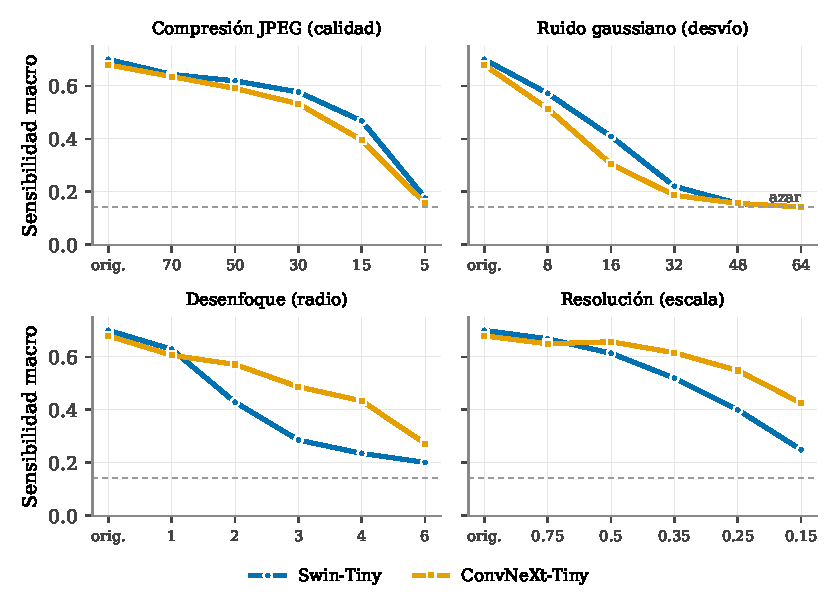
\includegraphics[width=0.85\textwidth]{Figures/Capitulos/04-Resultados-Clasificacion/robustez-curvas.pdf}
    \caption{Sensibilidad macro ante cuatro perturbaciones de intensidad creciente («orig.»: sin perturbar).}
    \label{fig:res_robustez}
\end{figure}

\begin{table}[H]
    \centering
    \caption{Caída relativa de la sensibilidad macro ante cuatro perturbaciones, por nivel de intensidad.}
    \label{tab:res_robustez}
    \small
    \setlength{\tabcolsep}{3pt}
    \begin{tabularx}{\textwidth}{@{}>{\raggedright\arraybackslash}X
        >{\centering\arraybackslash}p{1.1cm}>{\centering\arraybackslash}p{1.1cm}>{\centering\arraybackslash}p{1.1cm}
        >{\centering\arraybackslash}p{1.1cm}>{\centering\arraybackslash}p{1.1cm}>{\centering\arraybackslash}p{1.1cm}@{}}
        \toprule
        & \multicolumn{3}{c}{\textbf{Swin-Tiny}} & \multicolumn{3}{c}{\textbf{ConvNeXt-Tiny}} \\
        \cmidrule(lr){2-4}\cmidrule(l){5-7}
        \textbf{Perturbación (niveles 1, 3 y 5)} & \textbf{1} & \textbf{3} & \textbf{5} & \textbf{1} & \textbf{3}
            & \textbf{5} \\
        \midrule
        Compresión JPEG (calidad 70, 30 y 5) & 0.081 & 0.176 & 0.748 & 0.065 & 0.217 & 0.769 \\
        Ruido gaussiano (desvío 8, 32 y 64) & 0.184 & 0.685 & 0.796 & 0.244 & 0.725 & 0.790 \\
        Desenfoque (radio 1, 3 y 6) & 0.102 & 0.592 & 0.713 & 0.108 & 0.284 & 0.599 \\
        Resolución (0.75, 0.35 y 0.15) & 0.046 & 0.258 & 0.644 & 0.044 & 0.094 & 0.374 \\
        \bottomrule
    \end{tabularx}
\end{table}

Las degradaciones leves cuestan poco, salvo el ruido gaussiano, que es la perturbación más dañina: con un desvío de 8
sobre 255 ya quita casi un quinto de la sensibilidad macro, y en los niveles más altos lleva a los dos modelos al azar.
La compresión, en cambio, solo pesa cuando la calidad es muy baja. La diferencia más clara entre los dos modelos está
en el desenfoque y la reducción de resolución intensos, que ConvNeXt-Tiny soporta mejor. Estas perturbaciones
reproducen solo una parte de la variación real entre equipos (Sección~\ref{sec:marco_eval_robustez}), así que no
reemplazan la evaluación en \emph{HIBA}.

\subsection{Calibración}
\label{sec:res_calibracion}

Además de acertar la clase, el clasificador entrega probabilidades que fijan el umbral de melanoma y que un clínico
leería como certeza, y la tercera evaluación mide cuánto se puede confiar en ellas. La
Figura~\ref{fig:res_calibracion} muestra el diagrama de confiabilidad de Swin-Tiny con y sin pesos por clase, y la
Tabla~\ref{tab:res_calibracion} reúne el \gls{ece} y el Brier, también con los dos ajustes posteriores.

\begin{figure}[H]
    \centering
    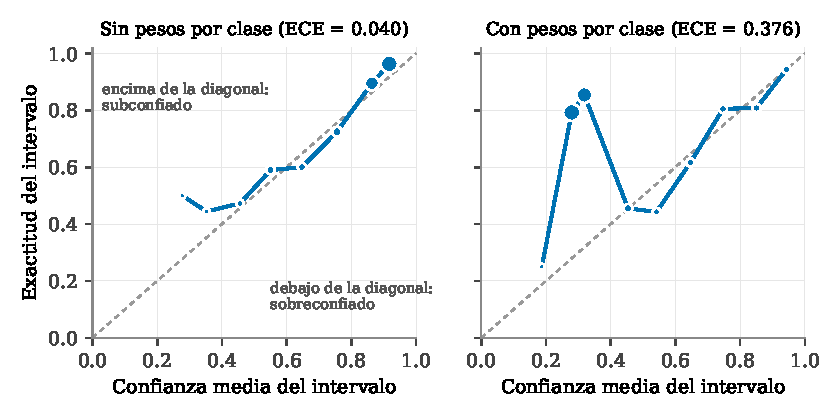
\includegraphics[width=0.85\textwidth]{Figures/Capitulos/04-Resultados-Clasificacion/calibracion-swin.pdf}
    \caption{Diagrama de confiabilidad de Swin-Tiny (semilla 42); el tamaño del punto es proporcional a la cantidad de imágenes del intervalo.}
    \label{fig:res_calibracion}
\end{figure}

\begin{table}[H]
    \centering
    \caption{Calibración en la prueba de \emph{HAM10000} (semilla 42). La fila con pesos por clase es la mejor configuración del barrido con pesos, distinta de la entropía cruzada ponderada de la Tabla~\ref{tab:res_desbalance}, que usa hiperparámetros fijos.}
    \label{tab:res_calibracion}
    \small
    \setlength{\tabcolsep}{4pt}
    \begin{tabularx}{\textwidth}{@{}>{\raggedright\arraybackslash}X
        >{\centering\arraybackslash}p{1.2cm}>{\centering\arraybackslash}p{1.2cm}>{\centering\arraybackslash}p{2.1cm}
        >{\centering\arraybackslash}p{1.2cm}>{\centering\arraybackslash}p{1.2cm}>{\centering\arraybackslash}p{2.1cm}@{}}
        \toprule
        & \multicolumn{3}{c}{\textbf{Swin-Tiny}} & \multicolumn{3}{c}{\textbf{ConvNeXt-Tiny}} \\
        \cmidrule(lr){2-4}\cmidrule(l){5-7}
        \textbf{Versión} & \textbf{ECE} & \textbf{Brier} & \textbf{Sensibilidad macro} & \textbf{ECE} & \textbf{Brier}
            & \textbf{Sensibilidad macro} \\
        \midrule
        Sin calibrar & 0.040 & 0.233 & 0.716 & 0.040 & 0.231 & 0.694 \\
        \emph{Temperature scaling} & 0.027 & 0.234 & 0.716 & 0.027 & 0.231 & 0.694 \\
        \emph{Vector scaling} & 0.014 & 0.216 & 0.675 & 0.033 & 0.226 & 0.687 \\
        \filasep
        Con pesos por clase & 0.376 & 0.609 & 0.770 & 0.211 & 0.636 & 0.742 \\
        \bottomrule
    \end{tabularx}
\end{table}

Sin pesos por clase, la curva sigue de cerca la diagonal, apenas por encima: el modelo es levemente subconfiado, es
decir, acierta algo más de lo que su confianza indica. Por eso la temperatura que ajusta la validación es menor que
uno, y con ella el \gls{ece} baja sin que cambie ninguna predicción. El vector scaling lo baja todavía más, pero
ajusta un parámetro por clase, cambia predicciones y reduce la sensibilidad macro. Con pesos por clase, en cambio, la
calibración se desarma: la confianza media cae a alrededor de 0.4 mientras la exactitud se mantiene cerca de 0.78, y
el \gls{ece} crece casi diez veces. En consecuencia, las probabilidades del modelo sin pesos pueden usarse casi sin
corrección, y las del modelo con pesos no deben leerse como certezas.

\subsection{Interpretabilidad}
\label{sec:res_interpretabilidad}

La última evaluación examina en qué parte de la imagen se apoya Swin-Tiny para decidir. La
Figura~\ref{fig:res_gradcam} muestra el mapa de Grad-CAM de la primera imagen de cada clase en la prueba. En las cinco
imágenes que el modelo clasifica bien (\gls{bkl}, \gls{df}, \gls{mel}, \gls{nv} y \gls{akiec}), la activación se
concentra sobre la lesión. De los dos errores, el \gls{bcc} clasificado como \gls{mel} también activa la lesión, lo
que sugiere una confusión entre lesiones pigmentadas y no una decisión tomada sobre el fondo. El \gls{vasc}
clasificado como \gls{nv}, en cambio, tiene una activación difusa sobre la piel que rodea la lesión. Como se trata de
siete imágenes, la inspección muestra que el modelo puede apoyarse en la lesión, pero no mide con qué frecuencia lo
hace ni prueba un razonamiento clínico (Sección~\ref{sec:met_interpretabilidad}).

\begin{figure}[H]
    \centering
    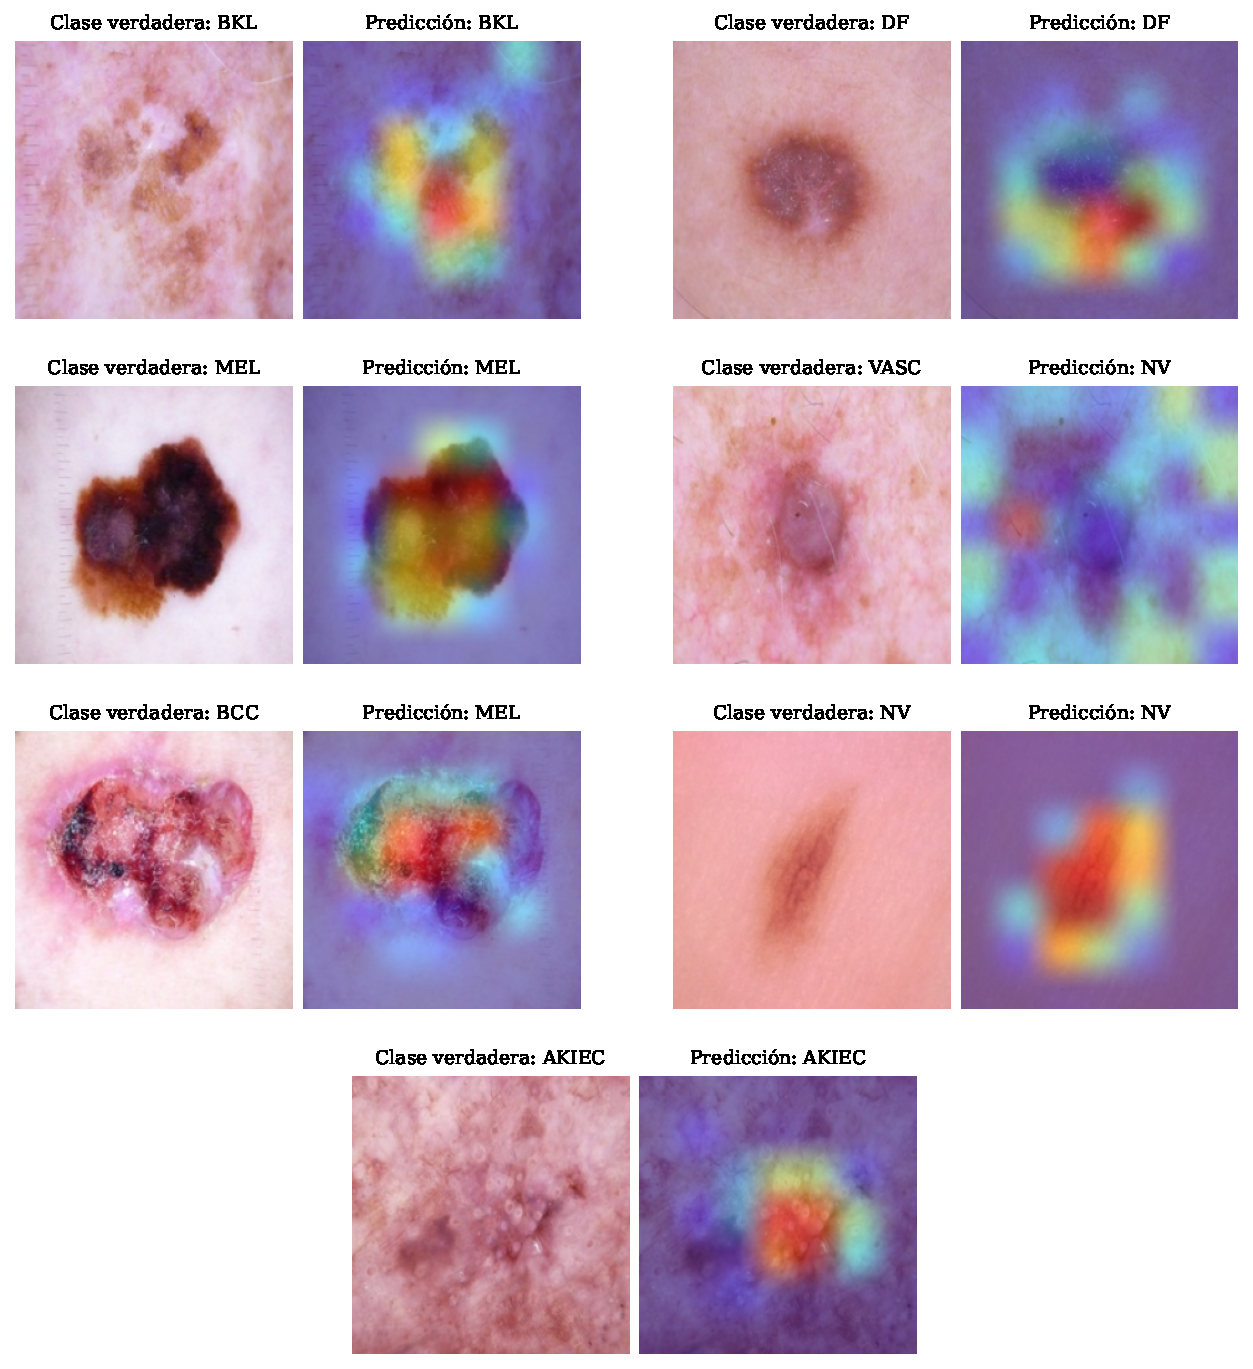
\includegraphics[width=0.9\textwidth]{Figures/Capitulos/04-Resultados-Clasificacion/gradcam-swin.pdf}
    \caption{Grad-CAM de Swin-Tiny sobre la primera imagen de prueba de cada clase.}
    \label{fig:res_gradcam}
\end{figure}

Con estas cuatro evaluaciones, el clasificador queda caracterizado también fuera de las condiciones de su
entrenamiento: pierde buena parte de su desempeño en otra población, es sensible al ruido de la imagen y entrega
probabilidades bien calibradas cuando se entrena sin pesos. Queda por ver si un \gls{vlm} podría ocupar su lugar, que es
lo que evalúa la sección siguiente.
